%========================================================================
% Modelo para elaboracao de textos academicos: TCC, dissertacoes e teses
% Elaborado pelo GISIS - Grupo de Imageamento Sismico e Inversao Sismica.
%========================================================================
\chapter{Metodologia}
\label{ch:metodologia}

Todas as informações dos experimentos realizados para verificar a precisão e a performance dos métodos de resolução da equação eikonal estão descritas neste capítulo. Começando pela comparação de precisão e performance utilizando modelos de propriedades simples e complexos, para averiguar a precisão em um modelo homogêneo, em um modelo de duas camadas e em um modelo complexo amplamente utilizado em análises sísmicas. Os resultados de performance são gerados no mesmo computador tendo um processador Intel i7-12700 com 20 núcleos e uma placa gráfica NVIDIA GeForce RTX 3060 com 12 GB de armazenamento. O sistema operacional Windows 11 é utilizado com a virtualização da distribuição linux Ubuntu via WSL.  

\section{Aplicação em modelo homogêneo}

Um modelo homogêneo foi aplicado com velocidade constante de 2000 m/s. O modelo tem 200 $\times$ 200 $\times$ 200 metros, com parâmetro de discretização de 1 m, totalizando 201 amostras em cada direção $x$, $y$ e $z$. A posição da fonte se encontra no centro do modelo. O tempo analítico é calculado a partir da distância da fonte a cada ponto da malha dividido pela velocidade do modelo. O erro é computado a partir da diferença entre o tempo numérico e o tempo analítico. As formulações de \citeonline{podvin1991finite}, \citeonline{jeong2008fast} e \citeonline{noble2014accurate} são analisadas. Como caso adicional, o operador mais preciso desenvolvido no trabalho de \citeonline{cai2023improved} é testado, pois o código foi fornecido pelo autor exatamente com um teste analítico nesse formado em questão. Na seção de resultados, somente a média e o máximo erro são mostrados assim como no trabalho de \citeonline{cai2023improved}. 

\section{Aplicação em modelo de refração}

Como parte de um experimento apresentado ao Simpósio Brasileiro de Geofísica \cite{alves2022refraction}, uma comparação numérica entre os métodos estudados será abordada, agora demonstrando a precisão no cálculo de ondas refratadas e o comportamento utilizando o princípio da reciprocidade. O exemplo esquemático aloca uma fonte na superfície do centro do modelo de velocidade e um arranjo circular de receptores espaçados regularmente de 50 metros com distância de 10 km da fonte. O modelo de velocidades empregado contém somente uma interface com propriedades de 1500 e 2000 m/s para cada camada. A figura \ref{fig:configurationNumericalComparison} mostra a configuração do experimento, o modelo de velocidades detalhado em forma de perfil e cortes do modelo com as isócronas de tempo projetadas. Para verificar a precisão dos métodos, foram construídos três modelos de velocidade com espaçamentos de 25, 50 e 100 metros. As amostras dos modelos construídos variam com a discretização do modelo sendo ($z$, $x$, $y$) = (12, 221, 221) amostras para o modelo de 100 m, (23, 441, 441) amostras para o modelo de 50 m e (45, 881, 881) amostras para o modelo de 25 m. Um estudo de reciprocidade, invertendo a posição da fonte com os receptores, foi efetuado para averiguar o funcionamento do algoritmo em larga escala. Assim, efeitos de inicialização em pontos fora da malha podem ser notados e o tempo de execução do problema para 1257 tiros pode ser registrado.

\begin{figure}[H]
	\centering
	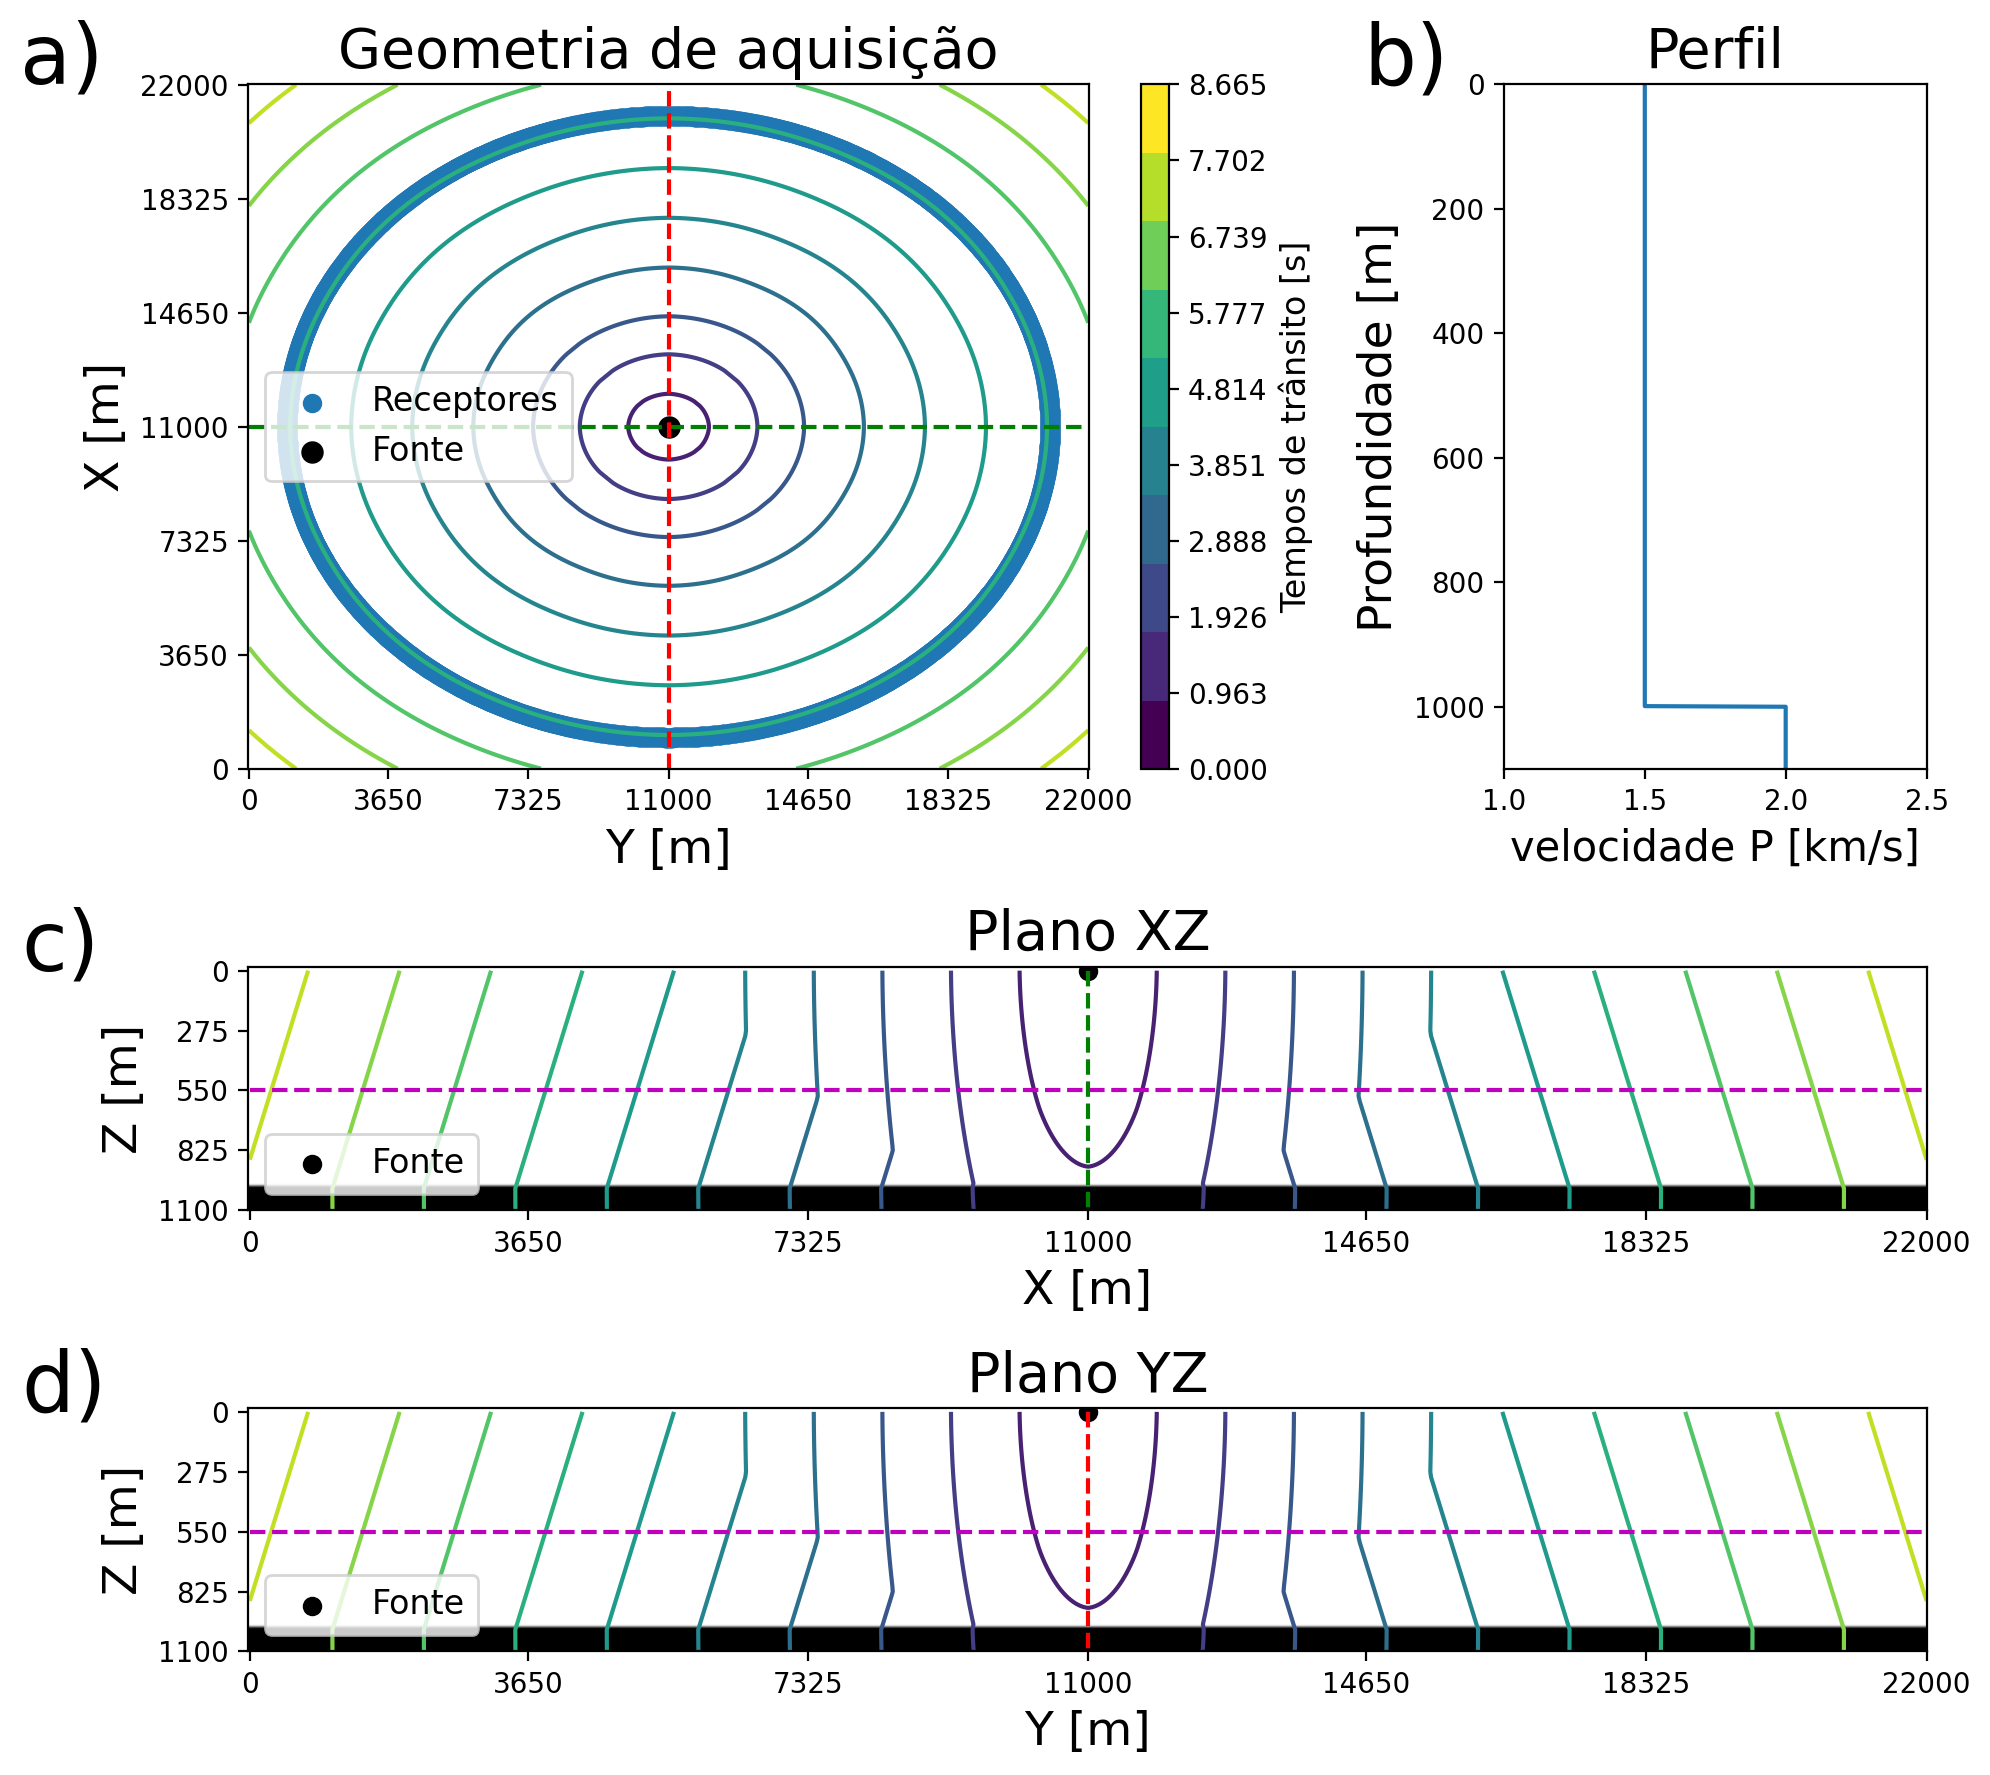
\includegraphics[width = 11cm, height = 11cm]{Imgs/RevisaoBibliografica/modelGeometry.png}
	\caption{Modelo empregado no teste de precisão e performance. (a) Plano XY ilustrando a geometria de aquisição com o arranjo de receptores circulares possuindo somente um tiro central. Isócronas mapeando o comportamento dos tempos de trânsito são mostradas. (b) Perfil de velocidades delimitando a posição da interface. (c) e (d) são as projeções dos cortes em planos XZ e YZ em relação à posição da fonte.}
	\label{fig:configurationNumericalComparison}
\end{figure}

\section{Aplicação em modelo complexo}

A fim de validar os algoritmos em um modelo realístico, as formulações estudadas foram aplicadas no modelo SEG/EAGE \textit{Overthrust}, ilustrado na Figura \ref{fig:overthrust}, na intenção de verificar o comportamento das frentes de onda e os tempos de execução perante uma simulação com altos contrastes de velocidade. O modelo possui dimensões de  ($z$, $x$, $y$) = (4.5, 20, 20) km e parâmetro de discretização de 25 m, totalizando (181, 801, 801) amostras. O esquema de geometria circular foi utilizado possuindo três círculos na superfície do modelo com afastamentos 5500, 7500 e 9500 metros do centro do modelo, onde a posição da fonte se encontra. O espaçamento entre os receptores é de 25 m, totalizando 5662 estações, para registrar o máximo de detalhes possível dos tempos gerados pelas formulações que resolvem a equação eikonal. Como o resultado desse experimento, as primeiras chegadas são apresentadas de forma geral e janelas de aproximação no dado mostram os detalhes que o modelo de alto contraste projeta nos dados calculados. Outro resultado são os tempos de execução das formulações de \citeonline{podvin1991finite}, \citeonline{jeong2008fast} e \citeonline{noble2014accurate} após o cálculo do tempo das ondas de primeira chegada. 

\begin{figure}[H]
	\centering
	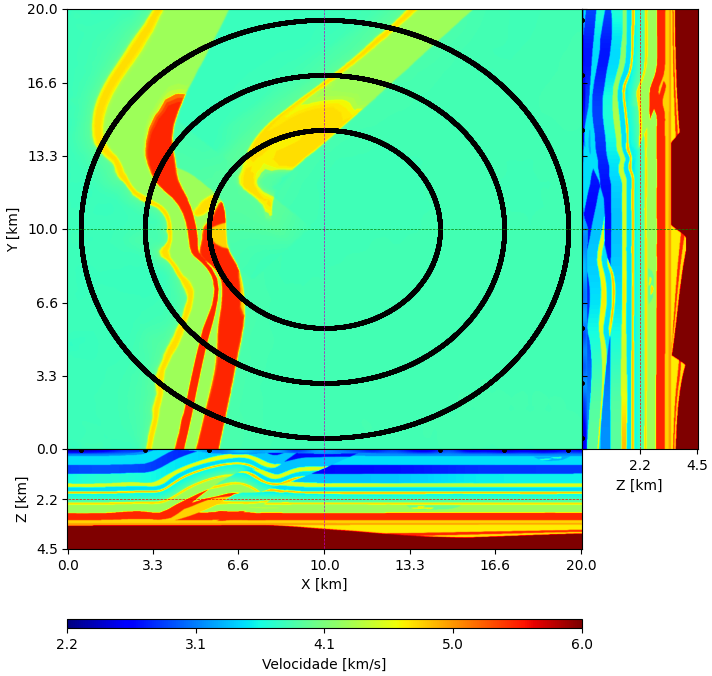
\includegraphics[width = 11cm, height = 9.99cm]{Imgs/Metodologia/overthrust.png}
	\caption{Modelo SEG/EAGE \textit{Overthrust} para aplicação dos métodos em altos contrastes de velocidade. A geometria circular é aplicada para verificar o comportamento azimutal dos tempos de trânsito. Em preto são os receptores espaçados em 25 metros totalizando 5662 estações. Uma fonte é a plicada no centro do modelo.}
	\label{fig:overthrust}
\end{figure}







